% Created 2014-09-19 金 20:15
\documentclass[t, aspectratio=169]{beamer}
\usepackage{zxjatype}
\usepackage[ipa]{zxjafont}
\setbeamertemplate{navigation symbols}{}
\hypersetup{colorlinks,linkcolor=,urlcolor=gray}
\AtBeginPart
{
  \begin{frame}<beamer|handout>
    \date{\insertpart}
    \maketitle
  \end{frame}
}
\AtBeginSection[]
{
  \begin{frame}<beamer>
  \tableofcontents[currentsection,currentsubsection]
  \end{frame}
}

\usepackage{minted}
\institute[AIIT]{産業技術大学院大学(AIIT)}
\usetheme{Berkeley}
\usecolortheme{seahorse}
\useinnertheme{rectangles}
\author{中鉢 欣秀 \\ yc@aiit.ac.jp}
\date{2014-09-22}
\title{ビジネスアプリケーション演習}
\hypersetup{
  pdfkeywords={},
  pdfsubject={},
  pdfcreator={Emacs 24.3.1 (Org mode 8.2.6)}}
\begin{document}

\maketitle

\part{第1章 [講義] ガイダンス}
\label{sec-1}
\section{自己紹介}
\label{sec-1-1}
\begin{frame}[label=sec-1-1-1]{自己紹介}
\begin{block}{名前}
\begin{itemize}
\item 中鉢 欣秀(ちゅうばち よしひで)
\end{itemize}
\end{block}
\begin{block}{出身地}
\begin{itemize}
\item 宮城県仙台市
\end{itemize}
\end{block}
\begin{block}{肩書}
\begin{itemize}
\item 産業技術大学院大学 産業技術研究科 \\ 情報アーキテクチャ専攻 准教授
\end{itemize}
\end{block}
\end{frame}
\begin{frame}[label=sec-1-1-2]{連絡先}
\begin{description}
\item[{E-Mail}] yc@aiit\ldots{}
\item[{Facebook}] ychubachi
\item[{Twitter}] ychubachi (あんまり使ってない)
\item[{Skype}] ychubachi (あんまり使ってない)
\end{description}
\end{frame}
\begin{frame}[label=sec-1-1-3]{学歴}
\begin{center}
\begin{tabular}{lll}
1991年 & 4月 & 慶應義塾大学環境情報学部 入学\\
1995年 & \alert{10月} & 同大大学院 政策・メディア研究科\\
 &  & 修士課程 入学\\
1997年 & 10月 & 同大大学院 政策・メディア研究科\\
 &  & 後期博士課程 入学\\
2004年 & 10月 & 同大大学院 政策・メディア研究科\\
 &  & 後期博士課程 卒業\\
 &  & 学位:博士(政策・メディア)\\
\end{tabular}
\end{center}
\end{frame}

\begin{frame}[label=sec-1-1-4]{職歴}
\begin{center}
\begin{tabular}{lll}
1997年 & 10月 & 合資会社ニューメリック設立\\
 &  & \alert{社長就任}\\
2005年 & 4月 & 独立行政法人科学技術振興機構\\
 &  & PD級研究員\\
 &  & (長岡技術科学大学)\\
2006年 & 4月 & 産業技術大学院大学 産業技術研究科\\
 &  & 情報アーキテクチャ専攻 准教授\\
\end{tabular}
\end{center}
\end{frame}
\begin{frame}[label=sec-1-1-5]{起業経験}
\begin{block}{社名}
\begin{itemize}
\item 合資会社ニューメリック
\end{itemize}
\end{block}
\begin{block}{設立}
\begin{itemize}
\item 1997年
\end{itemize}
\end{block}
\begin{block}{資本金}
\begin{itemize}
\item \alert{18万円}
\end{itemize}
\end{block}
\end{frame}
\begin{frame}[label=sec-1-1-6]{起業の背景}
\begin{block}{設立当時の状況}
\begin{itemize}
\item Windows 95が普及(初期状態でインターネットは使えなかった)
\item 後輩のやっていたベンチャーの仕事を手伝って面白かった
\end{itemize}
\end{block}
\begin{block}{会社設立の理由}
\begin{itemize}
\item 「やってみたかった」から
\item 少しプログラムがかければ仕事はいくらでもあった
\item 後輩にそそのかされた・笑
\end{itemize}
\end{block}
\end{frame}
\begin{frame}[label=sec-1-1-7]{起業から学んだこと}
\begin{itemize}
\item 実プロジェクトの経験
\item 使える技術
\item お金は簡単には儲からない
\end{itemize}
\end{frame}
\begin{frame}[label=sec-1-1-8]{教育における関心事}
\begin{block}{情報技術産業の変化}
\begin{itemize}
\item 情報技術のマーケットが変化
\item ユーザ・ベンダ型モデルの終焉
\end{itemize}
\end{block}
\begin{block}{モダンなソフトウエア開発者}
\begin{itemize}
\item 新しいサービスの企画から,ソフトウエアの実装まで何でもこなせる開発者
\item このような人材の育成方法
\end{itemize}
\end{block}
\end{frame}
\section{授業の全体像}
\label{sec-1-2}
\begin{frame}[label=sec-1-2-1]{学習目標と目的}
\begin{block}{目標}
\begin{itemize}
\item ビジネスアプリケーションを構築するための基礎力
\item 分散型PBLを実施する上で必要となる知識やツールの使い方
\item これら活用するための自己組織的なチームワーク
\end{itemize}
\end{block}
\begin{block}{目的}
\begin{itemize}
\item 分散ソフトウェア開発のための道具を学ぶ
\begin{itemize}
\item 開発環境(Ruby),VCSとリモートリポジトリ(GitHub)
\item テスト自動化,継続的インテグレーション,PaaS
\end{itemize}
\end{itemize}
\end{block}
\end{frame}
\begin{frame}[label=sec-1-2-2]{前提知識と到達目標}
\begin{block}{前提とする知識}
\begin{itemize}
\item 情報系の学部レベルで基礎的な知識を持っていること
\end{itemize}
\end{block}
\begin{block}{最低到達目標}
\begin{itemize}
\item 授業で取り上げる各種ツールの基本的な使い方を身につける
\end{itemize}
\end{block}
\begin{block}{上位到達目標}
\begin{itemize}
\item 授業で取り上げる各種ツールの高度な使い方に習熟する.
\end{itemize}
\end{block}
\end{frame}
\begin{frame}[label=sec-1-2-3]{授業の形態}
\begin{block}{対面授業}
\begin{itemize}
\item 担当教員による講義・演習
\end{itemize}
\end{block}
\begin{block}{個人演習}
\begin{itemize}
\item 個人によるソフトウエア開発
\end{itemize}
\end{block}
\begin{block}{グループ演習}
\begin{itemize}
\item グループによるソフトウエア開発
\end{itemize}
\end{block}
\end{frame}
\section{授業の方法}
\label{sec-1-3}
\begin{frame}[label=sec-1-3-1]{講義・演習・課題}
\begin{block}{講義}
\begin{itemize}
\item ツールの説明
\item ツールの使い方
\end{itemize}
\end{block}
\begin{block}{演習}
\begin{itemize}
\item 個人でツールを使えるようになる
\item グループでツールを使えるようになる
\end{itemize}
\end{block}
\end{frame}
\begin{frame}[label=sec-1-3-2]{成績評価}
\begin{block}{課題}
\begin{itemize}
\item 個人でソフトウエアを作る
\item グループでソフトウエアを作る
\end{itemize}
\end{block}
\begin{block}{評価の方法}
\begin{itemize}
\item 課題提出と実技試験
\end{itemize}
\end{block}
\begin{block}{評価の観点}
\begin{itemize}
\item 分散PBLで役に立つ知識が習得できたかどうか
\end{itemize}
\end{block}
\end{frame}
\section{モダンなソフトウエア開発}
\label{sec-1-4}
\begin{frame}[label=sec-1-4-1]{ソフトウエア開発のための方法・言語・道具}
\begin{figure}[htb]
\centering
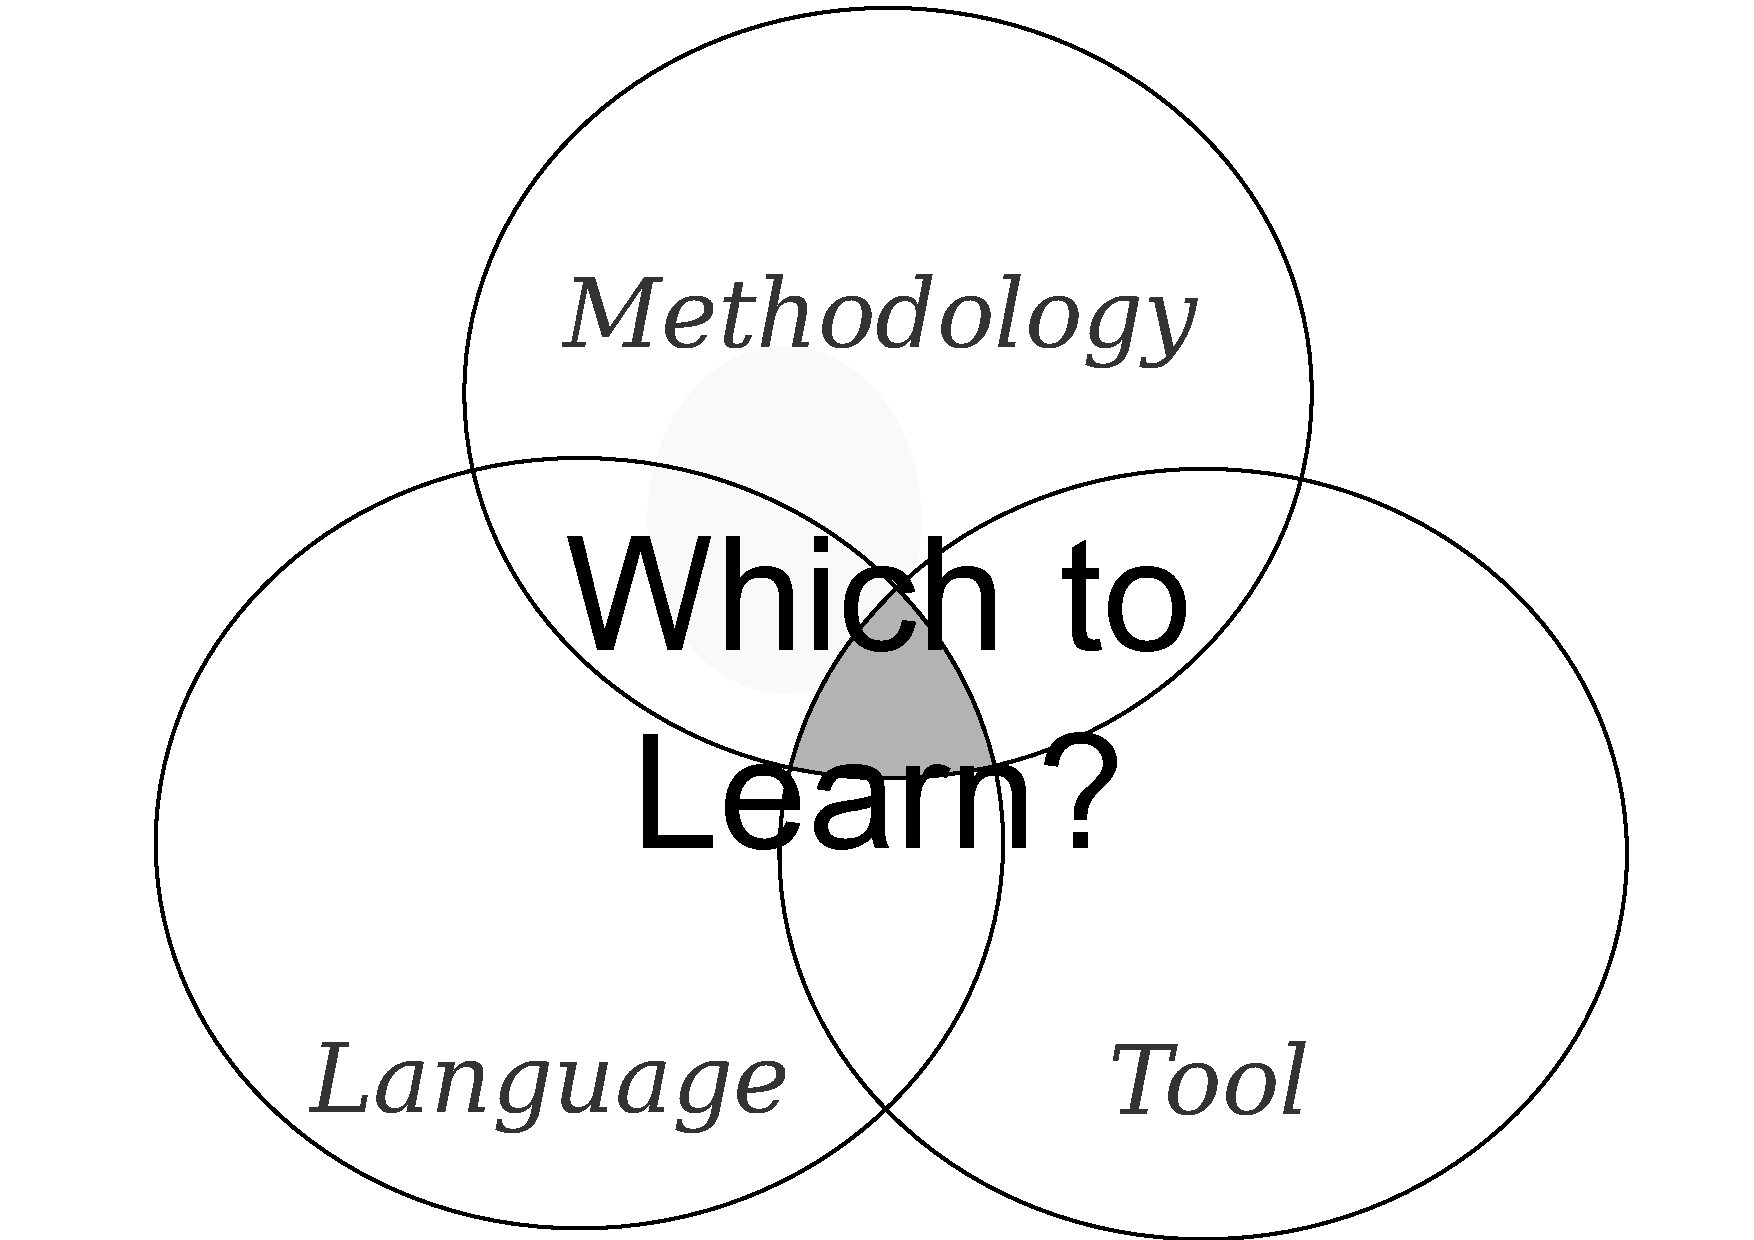
\includegraphics[width=0.6\textwidth]{./figures/FLT_framework.pdf}
\caption{\label{FLT_framework}The Framework-Language-Tool framework.}
\end{figure}
\end{frame}
\begin{frame}[label=sec-1-4-2]{授業で取り上げる範囲}
\begin{block}{取り上げること}
\begin{itemize}
\item 方法を支えるための道具
\item 良い道具には設計概念として方法論が組み込まれている
\item 道具はプログラミング言語を問わない
\end{itemize}
\end{block}
\begin{block}{取り扱わないこと}
\begin{itemize}
\item 方法論そのものについてはアジャイル開発特論で学ぶ
\item 言語の備えるエコシステムについては必要な範囲で学ぶ
\end{itemize}
\end{block}
\end{frame}
\begin{frame}[label=sec-1-4-3]{Scrumするための道具}
\begin{figure}[htb]
\centering
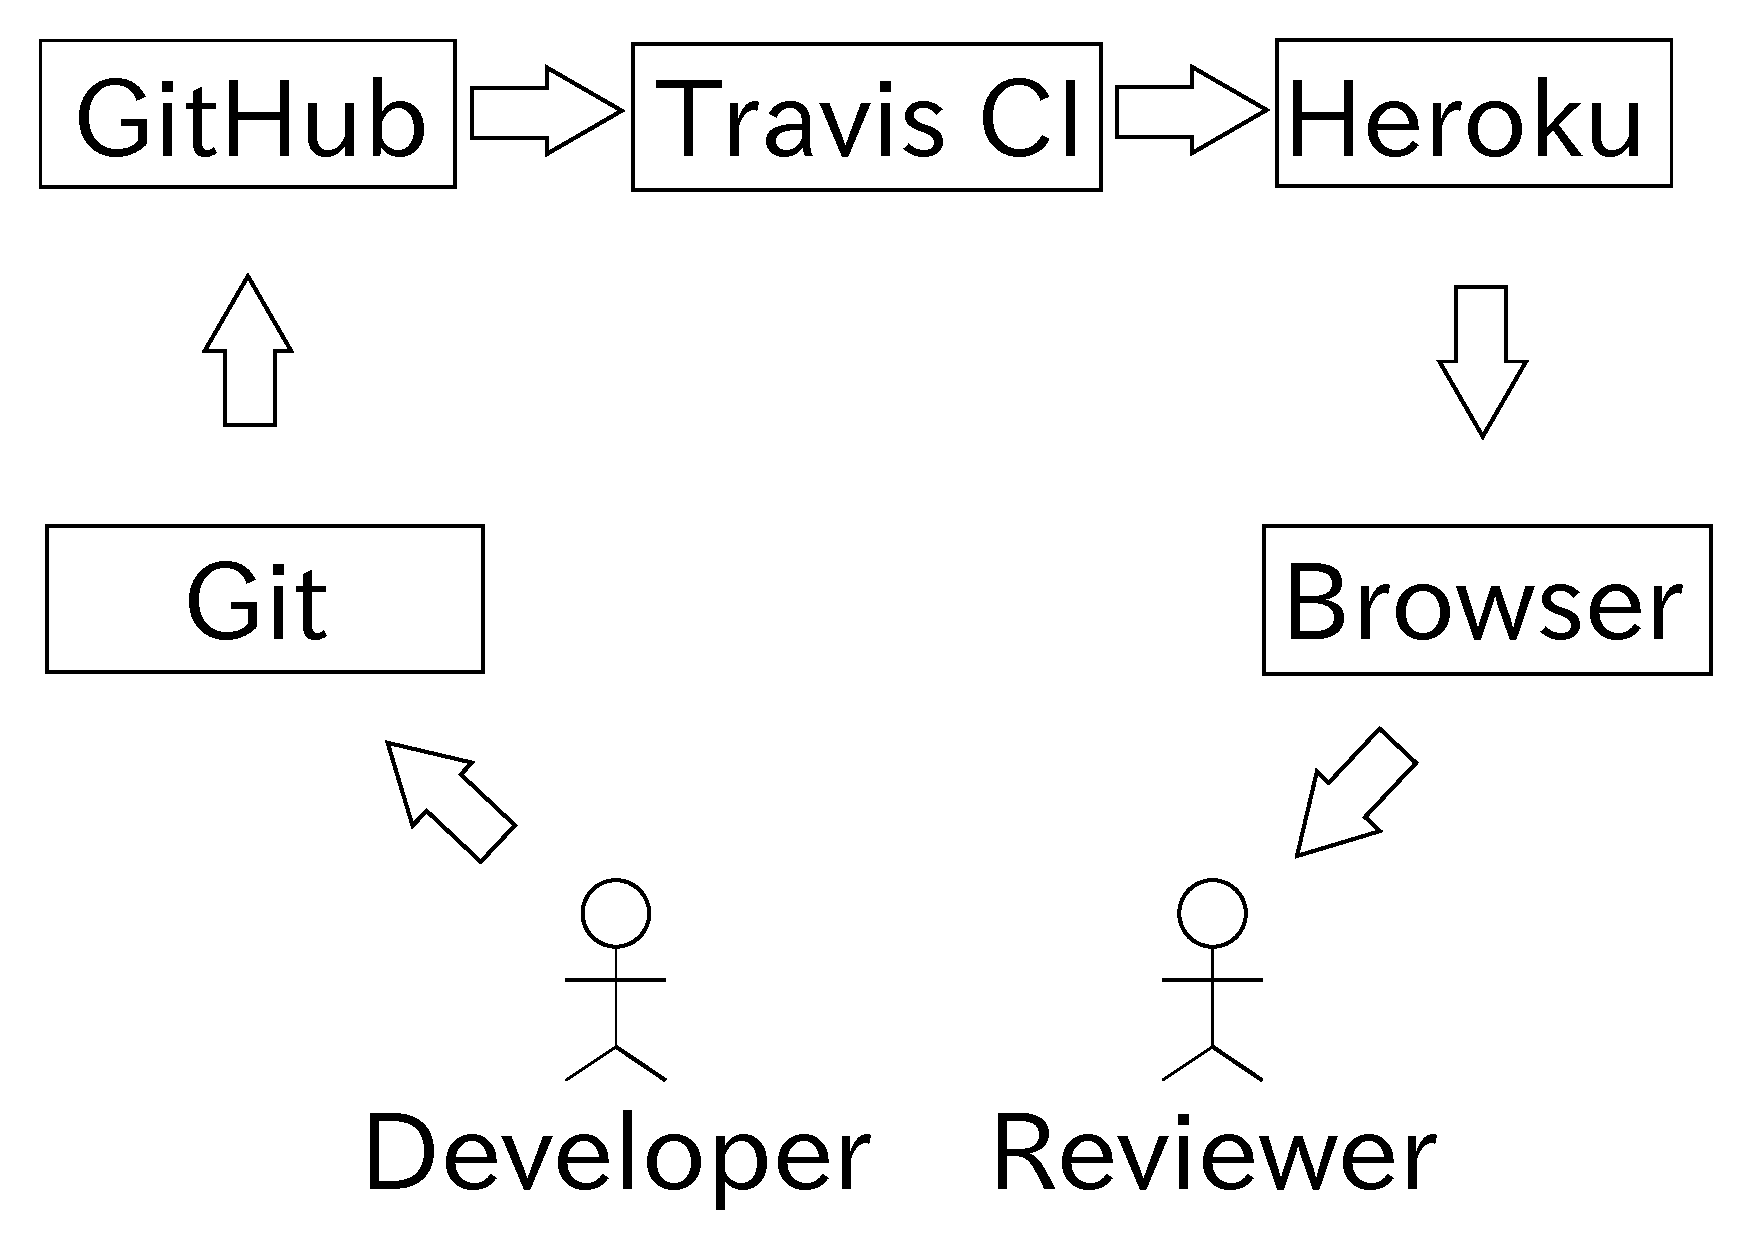
\includegraphics[width=0.6\textwidth]{./figures/tools.pdf}
\caption{\label{tools}The modern tools for Scrum developments.}
\end{figure}
\end{frame}

\begin{frame}[label=sec-1-4-4]{モダンな開発環境の全体像}
\begin{block}{仮想化技術(Virtualization)}
\begin{itemize}
\item WindowsやMacでLinux上でのWebアプリケーション開発を学ぶことができる
\item HerokuやTravis CI等のクラウドでの実行や検査環境として用いられている
\end{itemize}
\end{block}
\begin{block}{ソーシャルコーディング(Social Coding)}
\begin{itemize}
\item LinuxのソースコードのVCSとして用いられているGitを学ぶ
\item GitはGitHubと連携することでOSS型のチーム開発ができる
\end{itemize}
\end{block}
\end{frame}

\section{★演習課題(準備作業)★}
\label{sec-1-5}
\begin{frame}[label=sec-1-5-1]{クラウドのアカウント作成}
\begin{block}{GitHub}
\begin{itemize}
\item\relax [\href{https://github.com/join}{Join GitHub · GitHub}]
\end{itemize}
\end{block}
\begin{block}{Heroku}
\begin{itemize}
\item\relax [\href{https://id.heroku.com/signup}{Heroku - Sign up}]
\end{itemize}
\end{block}
\begin{block}{Travis CI}
\begin{itemize}
\item\relax [\href{https://travis-ci.org/}{Travis CI}]
\begin{itemize}
\item Travis CIは,GitHubのアカウントでログインできる
\end{itemize}
\end{itemize}
\end{block}
\end{frame}
\begin{frame}[fragile,label=sec-1-5-2]{enPiT仮想化環境のアップデート}
 \begin{block}{作業内容}
\begin{itemize}
\item enPiT仮想化環境(vagrantのbox)を更新しておく
\end{itemize}
\end{block}
\begin{block}{コマンド}
\begin{minted}[]{bash}
cd ~/enpit
vagrant destroy
vagrant box update
vagrant up
\end{minted}
\end{block}
\end{frame}

\begin{frame}[fragile,label=sec-1-5-3]{enPiT仮想化環境にログイン}
 \begin{block}{作業内容}
\begin{itemize}
\item 前の操作に引き続き,仮想化環境にSSH接続する
\end{itemize}
\end{block}
\begin{block}{コマンド}
\begin{minted}[]{bash}
vagrant ssh
\end{minted}
\end{block}
\end{frame}

\begin{frame}[label=sec-1-5-4]{github-connectスクリプト}
\begin{block}{URL}
\begin{itemize}
\item\relax [\href{https://gist.github.com/ychubachi/6491682}{github-connect.sh}]
\end{itemize}
\end{block}
\begin{block}{git conifgを代行}
\begin{itemize}
\item GitHubにログインし,名前とemailを読み込んでgitに設定
\end{itemize}
\end{block}
\begin{block}{SSHの鍵生成と登録}
\begin{itemize}
\item SSH鍵を作成し,公開鍵をGitHubに登録してくれる
\end{itemize}
\end{block}
\end{frame}
\begin{frame}[fragile,label=sec-1-5-5]{github-connect.shの実行}
 \begin{block}{作業内容}
\begin{itemize}
\item スクリプトを起動し,設定を行う
\item GitHubのログイン名とパスワードを聞かれるので,入力する
\item rsa key pairのパスフレーズは入力しなくて構わない
\end{itemize}
\end{block}
\begin{block}{コマンド}
\begin{minted}[]{bash}
github-connect.sh
\end{minted}
\end{block}
\end{frame}

\begin{frame}[fragile,label=sec-1-5-6]{GitとGitHubの設定確認}
 \begin{block}{Gitの設定確認}
\begin{minted}[]{bash}
git config --list
\end{minted}
\end{block}
\begin{block}{GitHubの設定確認}
\begin{itemize}
\item ブラウザでGitHubのSSH Keyページを開く
\end{itemize}
\end{block}
\end{frame}

\part{第2章 [講義] リポジトリの操作}
\label{sec-2}
\section{ローカルリポジトリ}
\label{sec-2-1}
\begin{frame}[fragile,label=sec-2-1-1]{Gitのローカルリポジトリの作成}
 \begin{block}{ローカルリポジトリ}
\begin{itemize}
\item ソースコードや各種のファイルを保存し,開発に利用する
\item 「 \texttt{my\_enpit} 」というディレクトリを作成し,初期化する
\end{itemize}
\end{block}
\begin{block}{コマンド}
\begin{minted}[]{bash}
mkdir ~/my_enpit
cd ~/my_enpit
git init
\end{minted}
\end{block}
\end{frame}

\begin{frame}[fragile,label=sec-2-1-2]{Gitの設定ディレクトリ}
 \begin{block}{隠しフォルダ「 \texttt{.git} 」}
\begin{itemize}
\item Gitソースコードの履歴情報や,各種の設定をGitが保存するディレクトリ
\item このフォルダは通常,Gitを経由しないで変更することはない
\end{itemize}
\end{block}
\begin{block}{確認方法}
\begin{minted}[]{bash}
ls -a
find .git
\end{minted}
\end{block}
\end{frame}

\section{リモートリポジトリ}
\label{sec-2-2}
\begin{frame}[fragile,label=sec-2-2-1]{Hubコマンド}
 \begin{block}{enPiT環境のHubコマンド}
\begin{itemize}
\item \href{https://github.com/github/hub}{github/hub}
\end{itemize}
\end{block}
\begin{block}{GitへのGitHub操作機能追加}
\begin{itemize}
\item 通常のGitの機能に加えて,GitHub用のコマンドが利用できる
\item エイリアス設定しており,コマンド名は「git」のまま
\end{itemize}
\end{block}
\begin{block}{確認方法}
\begin{minted}[]{bash}
git version
\end{minted}
\end{block}
\end{frame}

\begin{frame}[fragile,label=sec-2-2-2]{Hubコマンドによるリモートリポジトリの作成}
 \begin{block}{作業内容}
\begin{itemize}
\item コマンドライン操作で,GitHubにリポジトリを作成する
\item Hubコマンドの機能である \texttt{git create} を利用
\item 初回既動時にはパスワードか聞かれる
\end{itemize}
\end{block}
\begin{block}{コマンド}
\begin{minted}[]{bash}
git create
\end{minted}
\end{block}
\end{frame}

\begin{frame}[fragile,label=sec-2-2-3]{リポジトリの確認方法}
 \begin{block}{確認方法}
\begin{itemize}
\item WebブラウザでGitHubを開き,「 \texttt{my\_enpit} 」ができていることを確認
\end{itemize}
\end{block}
\begin{block}{コマンドラインで確認}
\begin{minted}[]{bash}
git remote -vv
\end{minted}
\end{block}
\end{frame}
\section{GitとGitHubの基本操作}
\label{sec-2-3}
\begin{frame}[label=sec-2-3-1]{Gitの操作方法}
\begin{block}{マニュアル等}
\begin{itemize}
\item \href{http://git-scm.com/doc}{Git - Documentation}
\end{itemize}
\end{block}
\begin{block}{commitログの書き方}
\begin{itemize}
\item \href{https://github.com/erlang/otp/wiki/Writing-good-commit-messages}{Writing good commit messages · erlang/otp Wiki}
\end{itemize}
\end{block}
\end{frame}
\begin{frame}[fragile,label=sec-2-3-2]{ステータスの確認}
 \begin{block}{リポジトリの状態を確認する}
\begin{itemize}
\item \texttt{git status} は,頻繁に利用するコマンド
\item リポジトリの状態を確認することができる
\item この表示の読み方を理解することが重要
\end{itemize}
\end{block}
\begin{block}{コマンド}
\begin{minted}[]{bash}
git status
\end{minted}
\end{block}
\end{frame}

\begin{frame}[fragile,label=sec-2-3-3]{ファイルの追加とステータスの確認}
 \begin{block}{作業内容}
\begin{itemize}
\item テキストエディタで \texttt{README.md} を作成
\item ステータスの変化を見る
\end{itemize}
\end{block}
\begin{block}{コマンド}
\begin{minted}[]{bash}
emacs README.md
git status
\end{minted}
\end{block}
\end{frame}

\begin{frame}[label=sec-2-3-4]{Add/Commitの方法}
\begin{block}{ステージングエリアを利用する場合}
\begin{itemize}
\item git add README.mb
\item git commit -m 'First commit'
\end{itemize}
\end{block}
\begin{block}{ステージングエリアを省略する場合}
\begin{itemize}
\item git commit -am 'First commit'
\end{itemize}
\end{block}
\end{frame}
\begin{frame}[fragile,label=sec-2-3-5]{Logの閲覧}
 \begin{block}{コミットログ}
\begin{itemize}
\item ソースコードに加えた変更の履歴を,commitを単位として閲覧できる
\end{itemize}
\end{block}
\begin{block}{コマンド}
\begin{minted}[]{bash}
git log
\end{minted}
\end{block}
\end{frame}

\begin{frame}[fragile,label=sec-2-3-6]{Pushの方法}
 \begin{block}{pushとは?}
\begin{itemize}
\item ローカルで作成したcommitを,リモートのリポジトリにアップロードすること
\item originとは,リモートのリポジトリの内部的な名前
\item upstreamとは,ブランチ(後述)が紐づいているリポジトリのこと
\item 最初にそのブランチをpushするときは, \texttt{-{}-setupstream} オプションを指定
\end{itemize}
\end{block}
\begin{block}{コマンド}
\begin{minted}[]{bash}
git push --set-upstream origin master
\end{minted}
\end{block}
\end{frame}

\section{★演習課題★}
\label{sec-2-4}
\begin{frame}[label=sec-2-4-1]{Init/Status/Addの練習}
\begin{block}{my\_enpitリポジトリの作成}
\begin{enumerate}
\item 解説した手順に従い,my\_enpitリポジトリを作成
\item git statusコマンドを実行
\item README.mdファイルを作成しなさい
\item git statusコマンドを実行し,変化を見なさい
\item commitしなさい.ログを必ず書くこと
\item git statusコマンドを実行し,変化を見なさい
\end{enumerate}
\end{block}
\end{frame}
\begin{frame}[fragile,label=sec-2-4-2]{Commit/Log/Pushの練習}
 \begin{block}{my\_enpitリポジトリで下記の作業を行う}
\begin{enumerate}
\item README.mdを修正してcommitしなさい
\item 新しいファイルを作成してcommitしなさい
\item 作業が完了したら,pushしなさい( \texttt{-{}-set-upstream} が必要)
\item コミットがpushされていることをWebブラウザで確認しなさい
\item 作成したファイルを削除してcommitしてpushしなさい
\item その他,いろいろとcommitの作業を試しなさい
\end{enumerate}
\end{block}
\end{frame}
\begin{frame}[label=sec-2-4-3]{ここまでの課題の提出}
\begin{block}{提出物}
\begin{itemize}
\item 下記のものを提出してください
\begin{itemize}
\item GitHubとHerokuアカウント
\item 作成したmy\_enpitリポジトリのURL
\end{itemize}
\end{itemize}
\end{block}
\begin{block}{提出先}
\begin{itemize}
\item\relax [\href{https://docs.google.com/forms/d/1SiKQqDLQw2YiJieYVS79ywpHIaNC3uI9cNPb_ddhC1Q/viewform?usp=send_form}{enPiT演習アカウント(2014)}]
\end{itemize}
\end{block}
\end{frame}

\part{第3章 ブランチの使い方リモートリポジトリでの協同作業}
\label{sec-3}
\section{ブランチの使い方}
\label{sec-3-1}
\begin{frame}[fragile,label=sec-3-1-1]{branchによる開発}
 \begin{block}{ブランチとは?}
\begin{itemize}
\item リポジトリにはmasterブランチがある
\item 新しい作業を行う場合,必ずbranchを切る
\end{itemize}
\end{block}
\begin{block}{コマンド}
\begin{minted}[]{bash}
git branch new_branch
git branch -vv
\end{minted}
\end{block}
\end{frame}

\begin{frame}[fragile,label=sec-3-1-2]{branchのcheckout}
 \begin{block}{branchを切り替える}
\begin{itemize}
\item checkoutしてブランチを切り替える
\item ブランチをcommitすることができる
\item 切り替える前に,ブランチでの作業はcommitしておく(stashも可)
\end{itemize}
\end{block}
\begin{block}{コマンド}
\begin{minted}[]{bash}
git checkout new_branch
<編集作業>
git commit -am 'Create a new branch'
\end{minted}
\end{block}
\end{frame}

\begin{frame}[fragile,label=sec-3-1-3]{他のbranchをmergeする}
 \begin{block}{mergeとは}
\begin{itemize}
\item ブランチで作業した内容(commit)を,他のブランチに統合すること
\item new\_branchでの作業をmasterに統合する場合,最初にmasterをcheckoutする
\end{itemize}
\end{block}
\begin{block}{コマンド操作}
\begin{minted}[]{bash}
git checkout master
git merge new_branch
\end{minted}
\end{block}
\end{frame}

\begin{frame}[label=sec-3-1-4]{Conflict(競合)とその解消}
\begin{block}{Conflictとは}
\begin{itemize}
\item branchで行う作業がかち合った場合,発生する
\item mergeする際,conflictが生じた場合,エラーになる
\end{itemize}
\end{block}
\begin{block}{解消方法}
\begin{itemize}
\item エディタ等で編集を行い,解消する
\end{itemize}
\end{block}
\end{frame}

\section{リモートのブランチとPull request}
\label{sec-3-2}
\begin{frame}[fragile,label=sec-3-2-1]{BranchのPush}
 \begin{block}{リモートへのPush}
\begin{itemize}
\item BranchをGitHubにPushすることができる
\item masterブランチをPushした際と同様,upstreamを指定する
\item PushできたかどうかをWebブラウザで確認する
\end{itemize}
\end{block}

\begin{block}{コマンド}
\begin{minted}[]{bash}
git push --set-upstream origin new_branch
\end{minted}
\end{block}
\end{frame}

\begin{frame}[fragile,label=sec-3-2-2]{Pull requestの作成}
 \begin{block}{Pull Roquestとは?}
\begin{itemize}
\item pushしたbranchでの作業の統合(merge)を依頼する
\item hubコマンドの \texttt{pull-request} で発行できる
\end{itemize}
\end{block}

\begin{block}{コマンド}
\begin{minted}[]{bash}
git pull-request -m 'Update a new branch'
\end{minted}
\end{block}
\end{frame}

\begin{frame}[label=sec-3-2-3]{Pull requestのmerge}
\begin{block}{Pull requestをレビューする}
\begin{itemize}
\item WebブラウザでPull requestを確認する
\end{itemize}
\end{block}
\begin{block}{ブラウザでmerge}
\begin{itemize}
\item 問題なければmergeボタンを押す
\end{itemize}
\end{block}
\begin{block}{コマンドラインでmergeする場合}
\end{block}
\end{frame}

\begin{frame}[fragile,label=sec-3-2-4]{BranchのPull}
 \begin{block}{BranchをPullするとは}
\begin{itemize}
\item リモートで行われた変更を適用すること
\item 内部的にはfetchでダウンロードしてからmergeする
\end{itemize}
\end{block}
\begin{block}{コマンド}
\begin{minted}[]{bash}
git checkout master
git pull
\end{minted}
\end{block}
\end{frame}

\section{★演習課題★}
\label{sec-3-3}
\begin{frame}[label=sec-3-3-1]{branchの操作}
\end{frame}
\begin{frame}[label=sec-3-3-2]{コミットのログ/Pull requestを丁寧に書く}
\end{frame}
\part{{\bfseries\sffamily WIP} }
\label{sec-4}
\section{{\bfseries\sffamily WIP} }
\label{sec-4-1}
\part{<演習> 開発環境の構築}
\label{sec-5}
\part{[講義] 道具の概要説明}
\label{sec-6}
\section{バージョン管理の概念}
\label{sec-6-1}
\begin{frame}[label=sec-6-1-1]{シナリオ}
\begin{block}{HTMLによるWebページ}
\end{block}
\begin{block}{index.htmlを作りブラウザで開く}
\end{block}
\end{frame}
\begin{frame}[label=sec-6-1-2]{バージョン管理の基礎知識}
\begin{block}{diff}
\end{block}
\begin{block}{patch}
\end{block}
\begin{block}{sha1}
\end{block}
\end{frame}
\section{Git}
\label{sec-6-2}
\begin{frame}[label=sec-6-2-1]{Gitコマンドの使い方}
\end{frame}
\begin{frame}[label=sec-6-2-2]{git status}
\end{frame}
\begin{frame}[label=sec-6-2-3]{git stageとcommit}
\end{frame}
\section{GitHub}
\label{sec-6-3}
\begin{frame}[label=sec-6-3-1]{GitHubのWeb管理画面}
\end{frame}
\begin{frame}[label=sec-6-3-2]{git pushとclone}
\end{frame}
\begin{frame}[label=sec-6-3-3]{ForkとPull Request}
\end{frame}
\begin{frame}[label=sec-6-3-4]{GitHubのその他の機能}
\end{frame}
\part{???もう一回講義増やす???}
\label{sec-7}
\section{Heroku}
\label{sec-7-1}
\begin{frame}[label=sec-7-1-1]{herokuのWeb管理画面}
\end{frame}
\begin{frame}[label=sec-7-1-2]{herokuコマンドによるdeploy}
\end{frame}
\section{Travis CI}
\label{sec-7-2}
\begin{frame}[label=sec-7-2-1]{Travis CIのWeb管理画面}
\end{frame}
\part{<演習> 静的サイトの開発演習(1)}
\label{sec-8}
\section{1人でやる演習}
\label{sec-8-1}
\begin{frame}[label=sec-8-1-1]{演習課題}
\begin{block}{演習課題}
\begin{itemize}
\item あなたがよく知っている「歴史上の有名人」を一人取り上げる
\item その人を紹介するWebページを作成する
\item HTMLを作成する(リンクや画像の埋め込みにもチャレンジ)
\item gitでバージョン管理
\item GitHubにpushする
\end{itemize}
\end{block}
\end{frame}
\begin{frame}[label=sec-8-1-2]{}
\end{frame}
\begin{frame}[label=sec-8-1-3]{GitHubでリポジトリを作成}
\end{frame}
\begin{frame}[label=sec-8-1-4]{Webページを作成してGitHubにpushする}
\end{frame}
\begin{frame}[label=sec-8-1-5]{作成した}
\end{frame}
\section{2人でやる演習}
\label{sec-8-2}
\begin{frame}[label=sec-8-2-1]{隣の人通しでPull Requestを送ってみる}
\end{frame}
\section{「GitHubによるソースコード共有」演習}
\label{sec-8-3}
\begin{frame}[label=sec-8-3-1]{}
\end{frame}
\section{「HTMLでのサイト構築」演習}
\label{sec-8-4}
\begin{frame}[label=sec-8-4-1]{演習の流れ}
\end{frame}
\begin{frame}[label=sec-8-4-2]{}
\end{frame}
\begin{frame}[label=sec-8-4-3]{2人でやる作業}
\end{frame}
\begin{frame}[label=sec-8-4-4]{グループでやる作業}
\end{frame}
\part{<演習> 動的サイトの開発演習(2)}
\label{sec-9}
\section{「Ruby(Sinatra)によるサイト構築」演習}
\label{sec-9-1}
\begin{frame}[label=sec-9-1-1]{演習の流れ}
\end{frame}
\section{Herokuでのテスト}
\label{sec-9-2}
\part{[講義] Ruby on Railsを用いた開発}
\label{sec-10}
\section{Ruby on Railsの全体像}
\label{sec-10-1}
\section{Scaffoldの作成と動作}
\label{sec-10-2}
\begin{frame}[label=sec-10-2-1]{Herokuへのdeploy}
\end{frame}
\begin{frame}[label=sec-10-2-2]{ScaffoldによるModelの拡張}
\end{frame}
\section{RSpecによるテスト}
\label{sec-10-3}
\begin{frame}[label=sec-10-3-1]{RSpecの実行}
\end{frame}
\begin{frame}[label=sec-10-3-2]{GitHubとTravis CI連携}
\end{frame}
\begin{frame}[label=sec-10-3-3]{Travis経由でのHerokuへのdeploy}
\end{frame}
\part{<演習> Ruby on Railsを用いた開発演習(1)}
\label{sec-11}
\part{<演習> Ruby on Railsを用いた開発演習(2)}
\label{sec-12}
\part{[講義] Web API活用したサービス構築}
\label{sec-13}
\section{楽天API}
\label{sec-13-1}
\part{<演習> Web API活用したサービス構築演習(1)}
\label{sec-14}
\part{<演習> Web API活用したサービス構築演習(2)}
\label{sec-15}
\part{[講義] ミニプロジェクト}
\label{sec-16}
\part{<演習> ミニプロジェクト演習(1)}
\label{sec-17}
\part{<演習> ミニプロジェクト演習(2)}
\label{sec-18}
\part{Tasks}
\label{sec-19}
\section{{\bfseries\sffamily DONE} chocolateyのインストールをkazamでキャプチャする}
\label{sec-19-1}
\section{{\bfseries\sffamily TODO} 英語の原典を読めるようになること}
\label{sec-19-2}
\section{{\bfseries\sffamily TODO} よくある間違い cdしないでgit initするとか.}
\label{sec-19-3}
\section{{\bfseries\sffamily TODO} OSをインストールし,手順書を参照しながら長々とコマンドを打つ,ということが不要になった.}
\label{sec-19-4}
\section{{\bfseries\sffamily TODO} アンケートを作成する}
\label{sec-19-5}
\begin{itemize}
\item 調査の目的
\begin{itemize}
\item モダンなソフトウエア開発の理解度(これは2回やる)
\begin{itemize}
\item gitについて
90\%(業務でのソフトウエア開発に利用できる)
  , 70\%, 50\%, 30\%,
10\% (ほとんど知らない・使ったことはない)
\end{itemize}
\item PBLのために,事前学習が役に立ったか(これはPBL後)
事前学習をした人とそうでない人とで,PBLの満足感,達成感が違うか
円滑にPBLをすすめることができたか
\end{itemize}

\item 方法論
\end{itemize}
あなたはBizApp演習の内容を学習しましか?
\begin{enumerate}
\item 授業を履修した
\begin{enumerate}
\item ビデオを視聴した
\begin{enumerate}
\item 学習していない
\end{enumerate}
\end{enumerate}
\item 道具
\end{enumerate}
\section{{\bfseries\sffamily TODO} .bash\_profileから.bashrcを読み込む(カラー化)}
\label{sec-19-6}
% Emacs 24.3.1 (Org mode 8.2.6)
\end{document}
